\documentclass{beamer}
\usetheme{Boadilla}
\usecolortheme{beaver}
%\usepackage{graphicx}
%\usepackage{minted}
%\usepackage[numbers]{natbib}
%\usepackage{float}
%\usepackage{multicol}
%\usepackage[magyar]{babel}
\usepackage{hyperref}
\usepackage{multimedia}
%\usepackage{comment}
%\usepackage{ragged2e}

\hypersetup{colorlinks=true, linkcolor=blue, filecolor=magenta, urlcolor=cyan}
\urlstyle{same}

\title[Jármű trajektóriák előrejelzése]{Járművek trajektóriáinak előrejelzése machine learning modellekkel}
\author{Péter Bence Mérnökinformatika BSc 6. félév\\Témavezetők:\\Dr. Horváth András egyetemi docens\\Agg Áron PhD hallgató}
\institute{Széchenyi István University}

\date{TMDK April 26, 2023}

\begin{document}

\begin{frame}
\titlepage
\end{frame}

\begin{frame}
\frametitle{Tartalom}
\tableofcontents
\end{frame}

\section{Bevezetés}
\begin{frame}{Bevezetés}
    \begin{itemize}
        \item Adathalmaz: 
        \begin{itemize}
            \item 5 különböző helyszín Amerikai városokból
            \item 10 órányi felvétel
        \end{itemize}
    \end{itemize}
    \centering
    %\includegraphics[scale=0.3]{deepsort_yolo_figs/gépilátás_modified.jpg}
    \movie[showcontrols=true]{\includegraphics[scale=0.3]{../deepsort_yolo_figs/gépilátás_modified.jpg}}{demo_bevezetes.mp4}
\end{frame}


\section{Objektumdetektálás}
\begin{frame}{Objektumdetektálás}
    \begin{columns}
        %TODO yolo jellemzes, sok felhasznalo, valos ideju futas ...
        \column{0.3\textwidth}
        \begin{figure}
            
\includegraphics[scale=0.05]{yolo_logo.png}
        \end{figure}
        \begin{itemize}
            \item A világon százezrek használják
            \item Nagy pontosság, valós időben egy erős videókártyán
        \end{itemize}

        \column{0.7\textwidth} 
        \centering
        \begin{figure}
            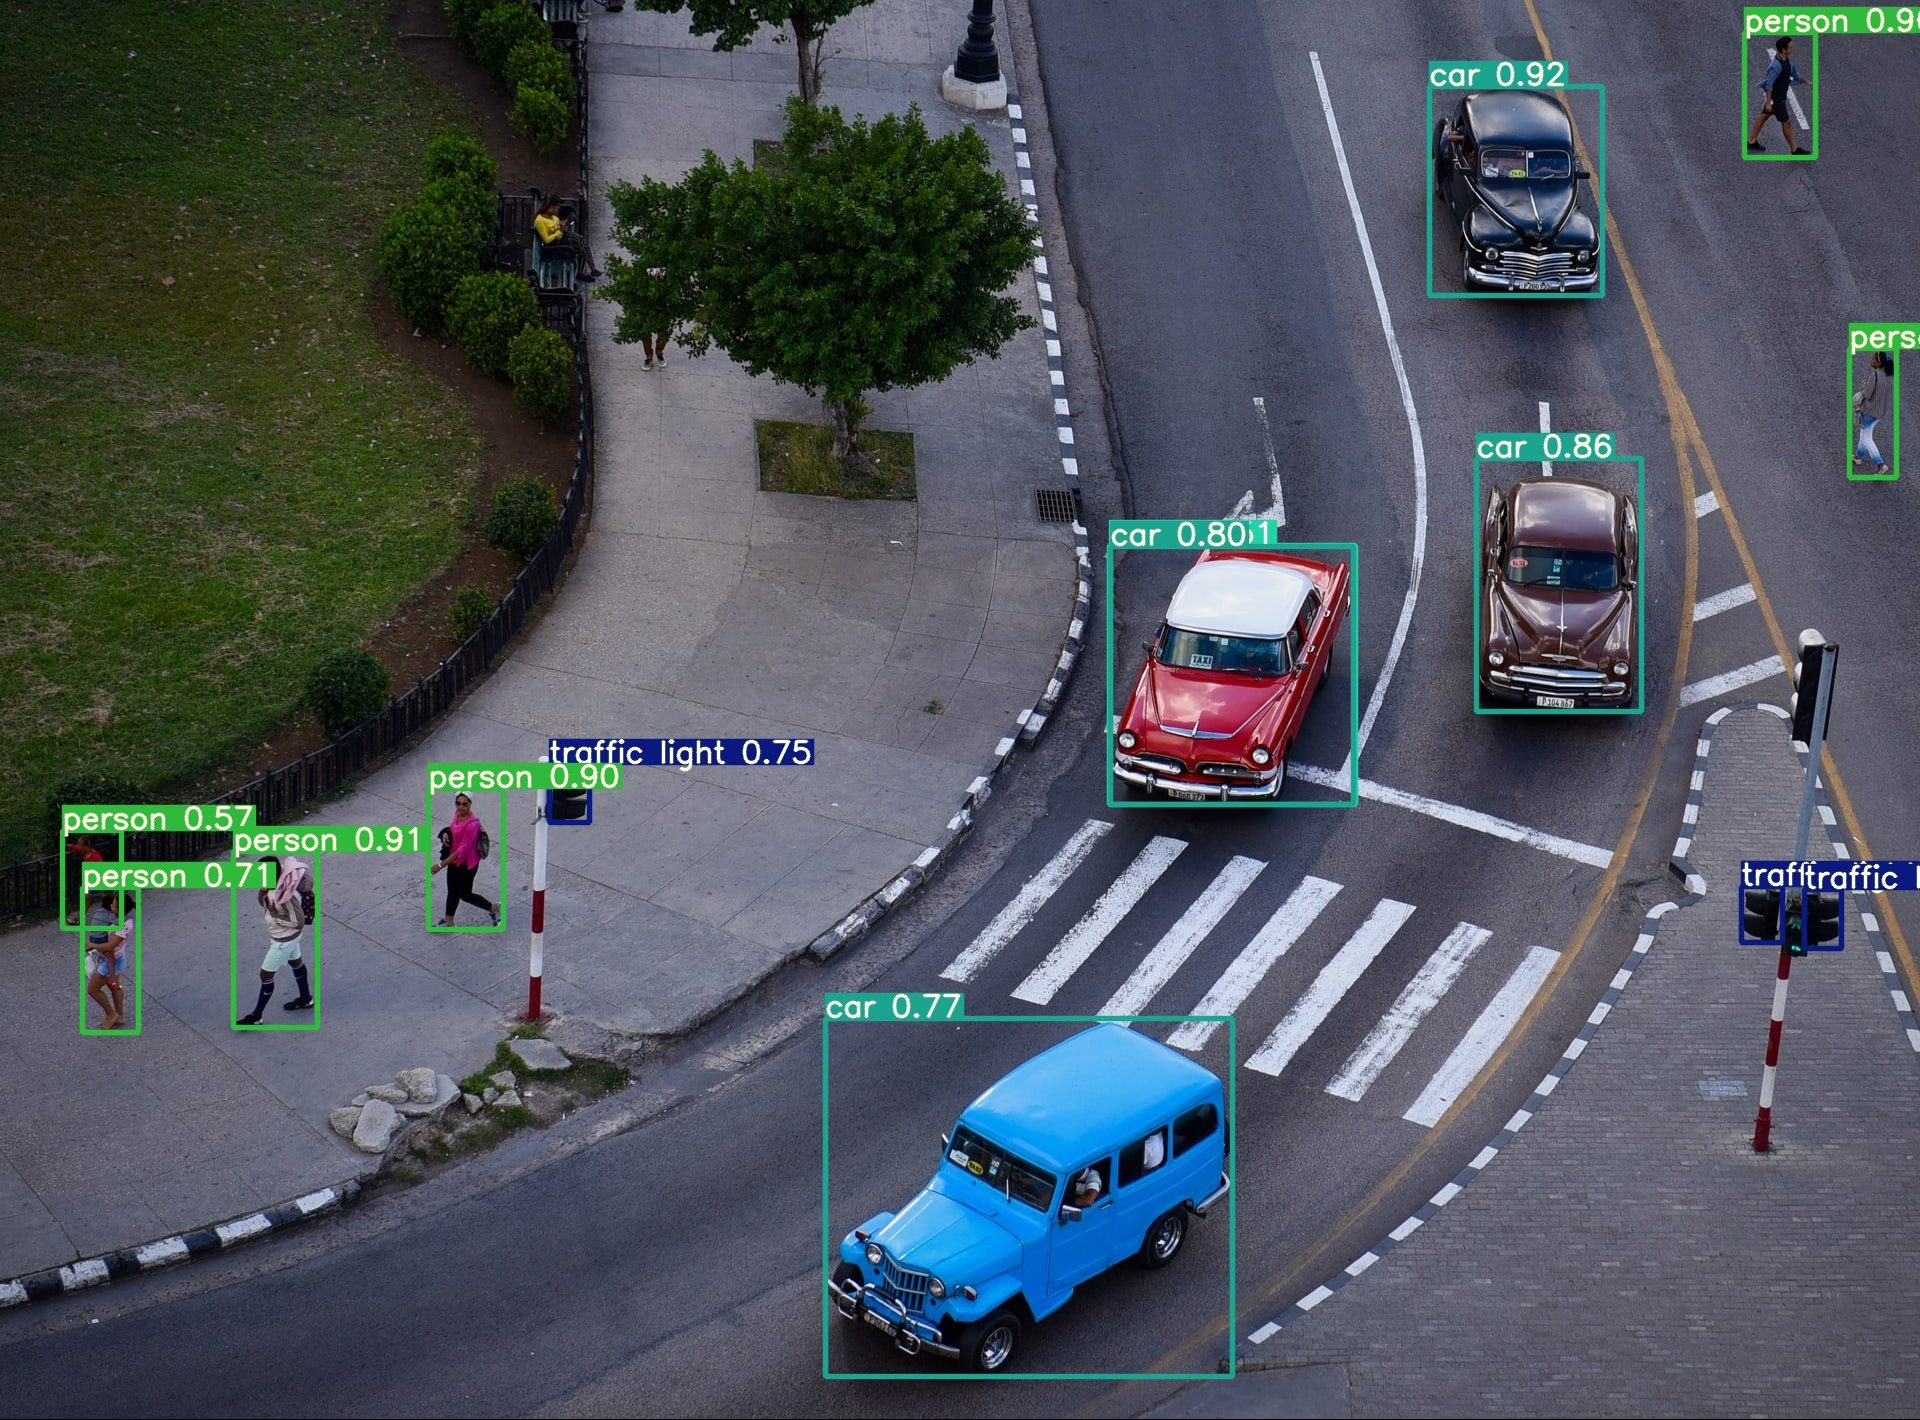
\includegraphics[scale=0.15]{yolo_img.jpg} 
        \end{figure}

    \end{columns}
\end{frame}

\section{Trajektória}
\begin{frame}{Trajektória}
   \begin{figure}
        \includegraphics[scale=0.15]{trajektoriak/car1_1.png}
        \includegraphics[scale=0.15]{trajektoriak/car1_2.png}
        \includegraphics[scale=0.15]{trajektoriak/car1_3.png}
        \includegraphics[scale=0.15]{trajektoriak/car1_4.png}
   \end{figure} 
   \begin{figure}
        \includegraphics[scale=0.2]{trajektoriak/car2_1.png}
        \includegraphics[scale=0.2]{trajektoriak/car2_2.png}
        \includegraphics[scale=0.2]{trajektoriak/car2_3.png}
        \includegraphics[scale=0.2]{trajektoriak/car2_4.png}
   \end{figure} 
\end{frame}

\section{Objektumkövetés}
\begin{frame}{Objektumkövetés}
    \centering
    \begin{figure}
        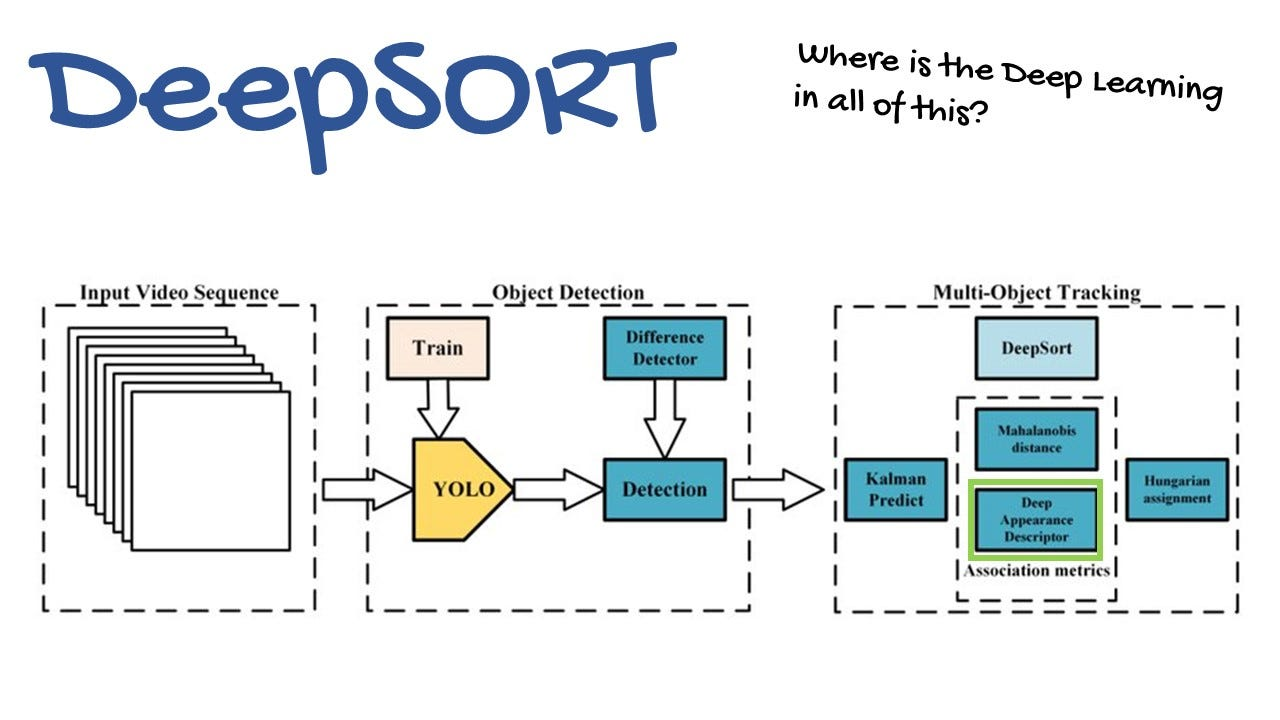
\includegraphics[scale=0.2]{deepsort_flowchart.jpg} 
    \end{figure}
    \begin{itemize}
        \item YOLO detektálások összefűzése trajektóriákká
    \end{itemize}
\end{frame}

\section{Machine Learning}
\begin{frame}{Machine Learning}
    \centering
    \begin{figure}
        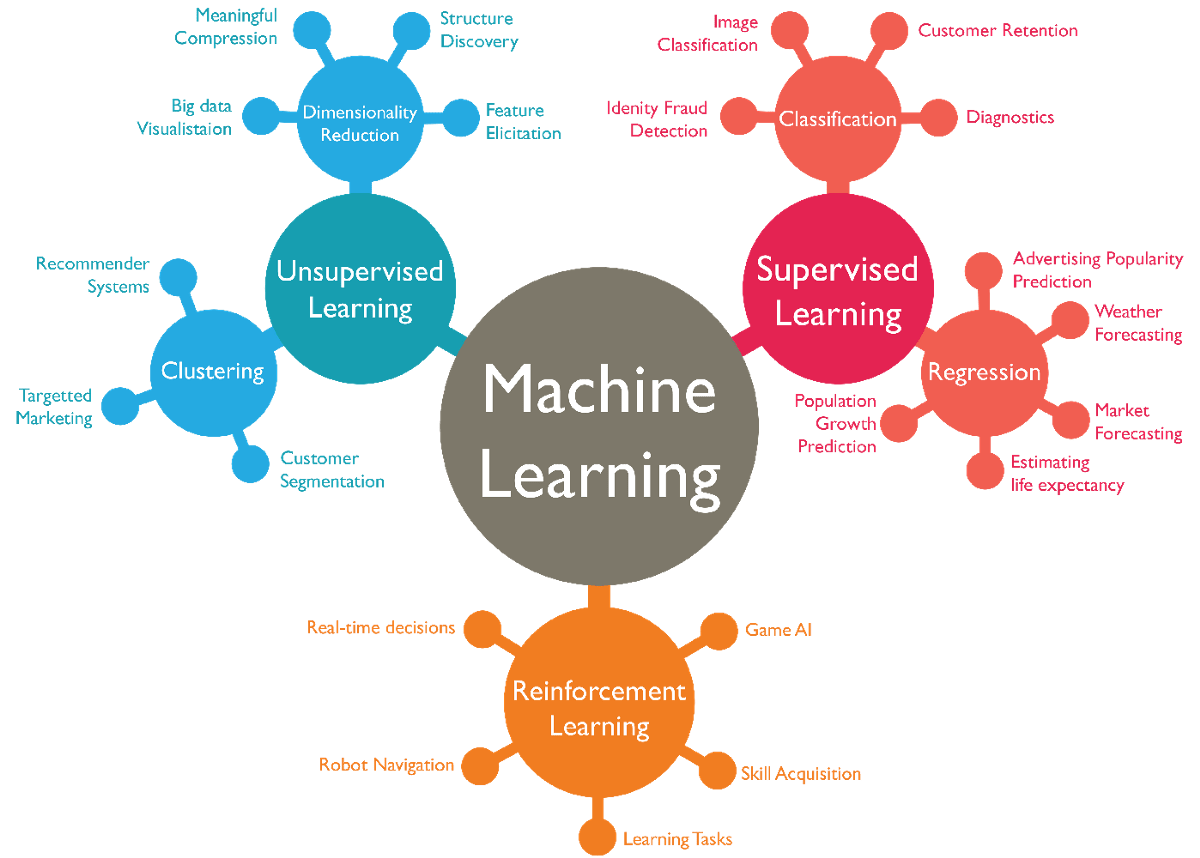
\includegraphics[scale=0.2]{machine_learning.png}    
    \end{figure}
\end{frame}
\subsection{Unsupervised learning (Nem felügyelt tanulás)}
\begin{frame}{Unsupervised learning (Nem felügyelt tanulás)}
    \begin{itemize}
        \item Nincsenek előre meghatározott osztályok
        \item Az algoritmus saját maga próbálja csoportokba rendezni a adatokat
    \end{itemize}
    \begin{figure}
        \includegraphics[scale=0.3]{unsupervised_learning.png}
    \end{figure}
\end{frame}
\subsection{Supervised learning (Felügyelt tanulás)}
\begin{frame}{Supervised learning (Felügyelt tanulás)}
    \begin{itemize}
        \item Előre meghatározott osztályok alapján
        \item Az algoritmust tanítani kell példa adatokkal 
        \item Amiket vagy kézzel, vagy klaszterezéssel rendezünk osztályokba
    \end{itemize}
    \begin{figure}
        \includegraphics[scale=0.25]{supervised_learning.jpeg}
    \end{figure}
\end{frame}

\section{Tipikus viselkedesi formak meghatarozasa: Klaszterezes (Unsupervised)}
\begin{frame}{Tipikus viselkedesi formak meghatarozasa: Klaszterezes (Unsupervised)}
    \begin{itemize}
        \item Bemeneti adatok: gyűjtött trajektóriák objektumdetektálás és követés segítségével
        \item Feature vektorok: trajektóriák be és kimeneti pontjai
    \end{itemize}
    \begin{columns}
        \column{0.33\textwidth}
        \begin{figure}
            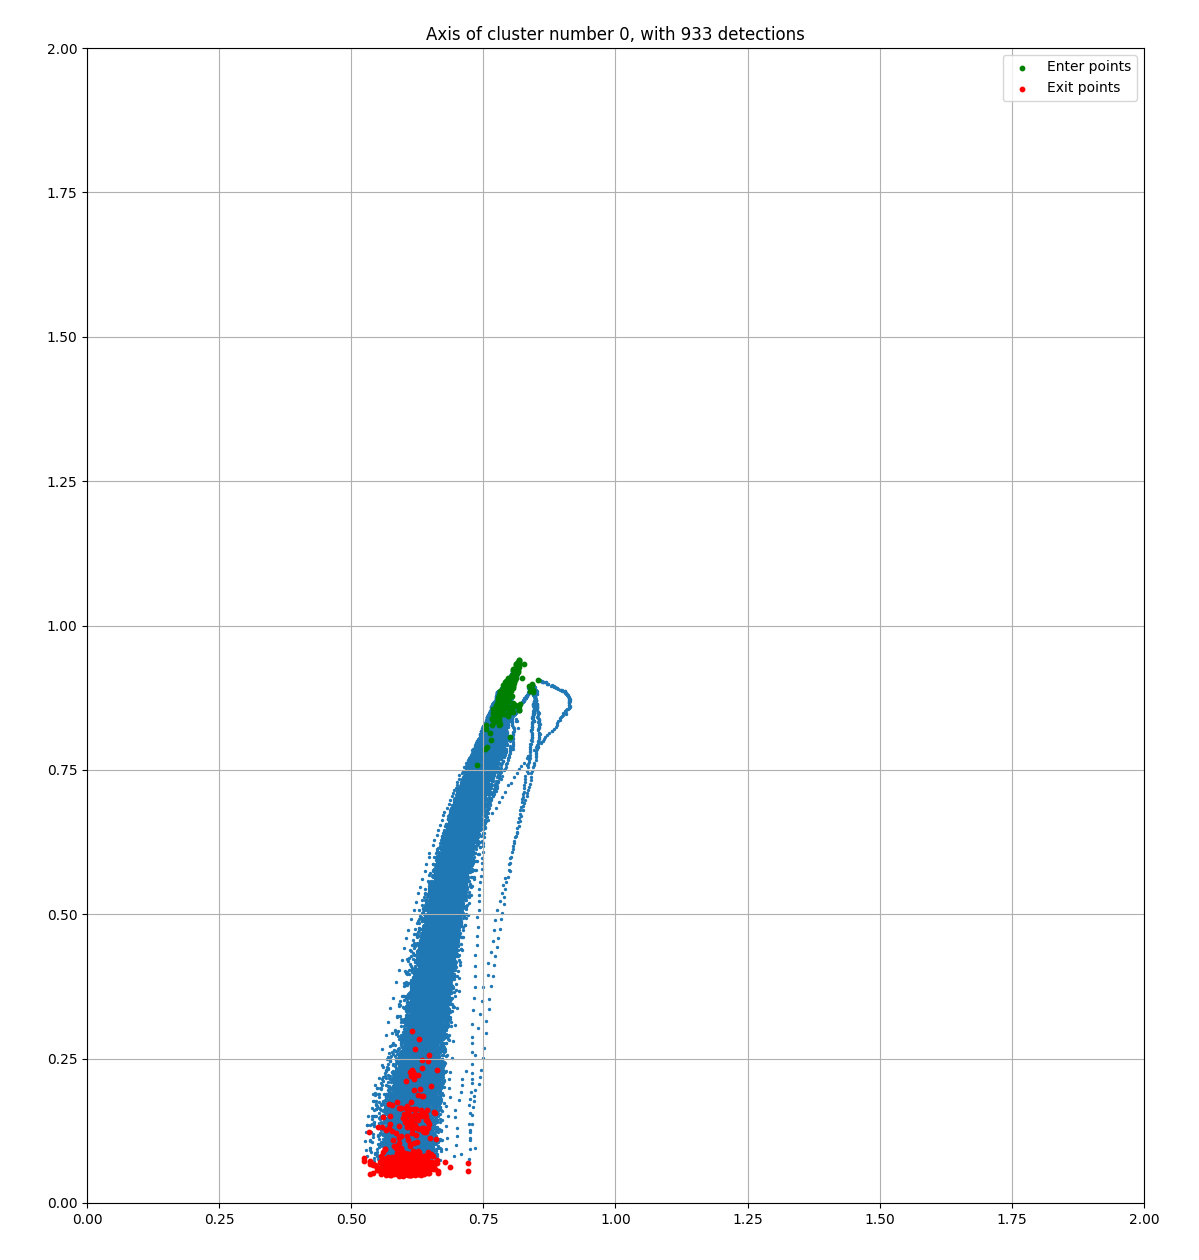
\includegraphics[scale=0.1]{../clustering/n_cluster_0_n_tracks_933_cropped.jpg}
        \end{figure}
        \column{0.33\textwidth}
        \begin{figure}
            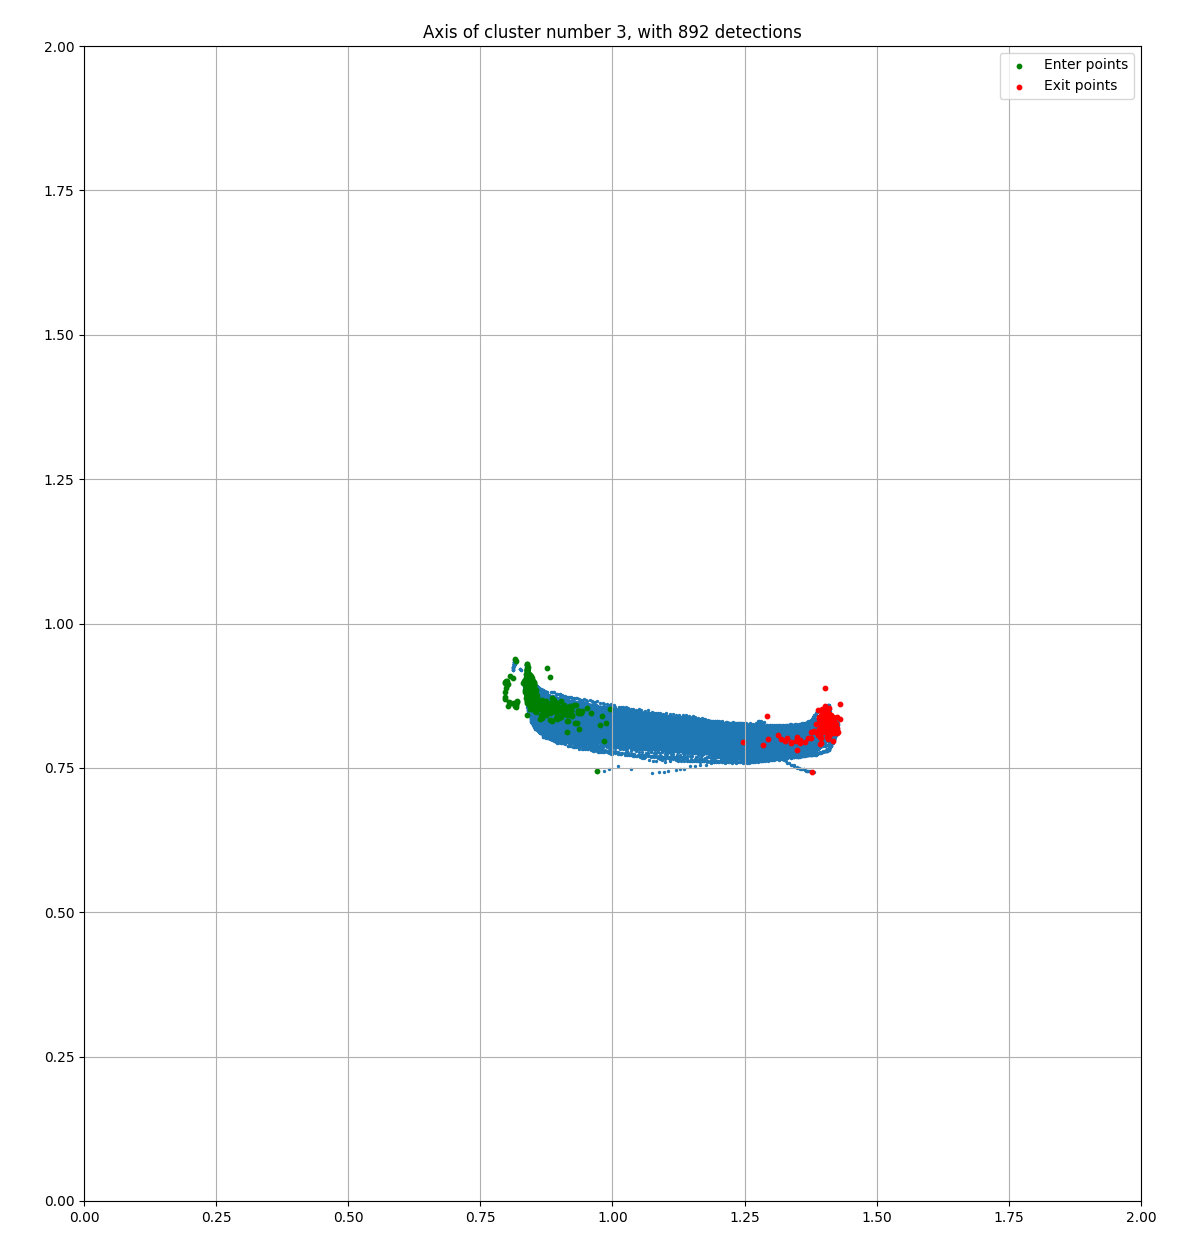
\includegraphics[scale=0.1]{../clustering/n_cluster_3_n_tracks_892_cropped.jpg}
        \end{figure}
        \column{0.33\textwidth}
        \begin{figure}
            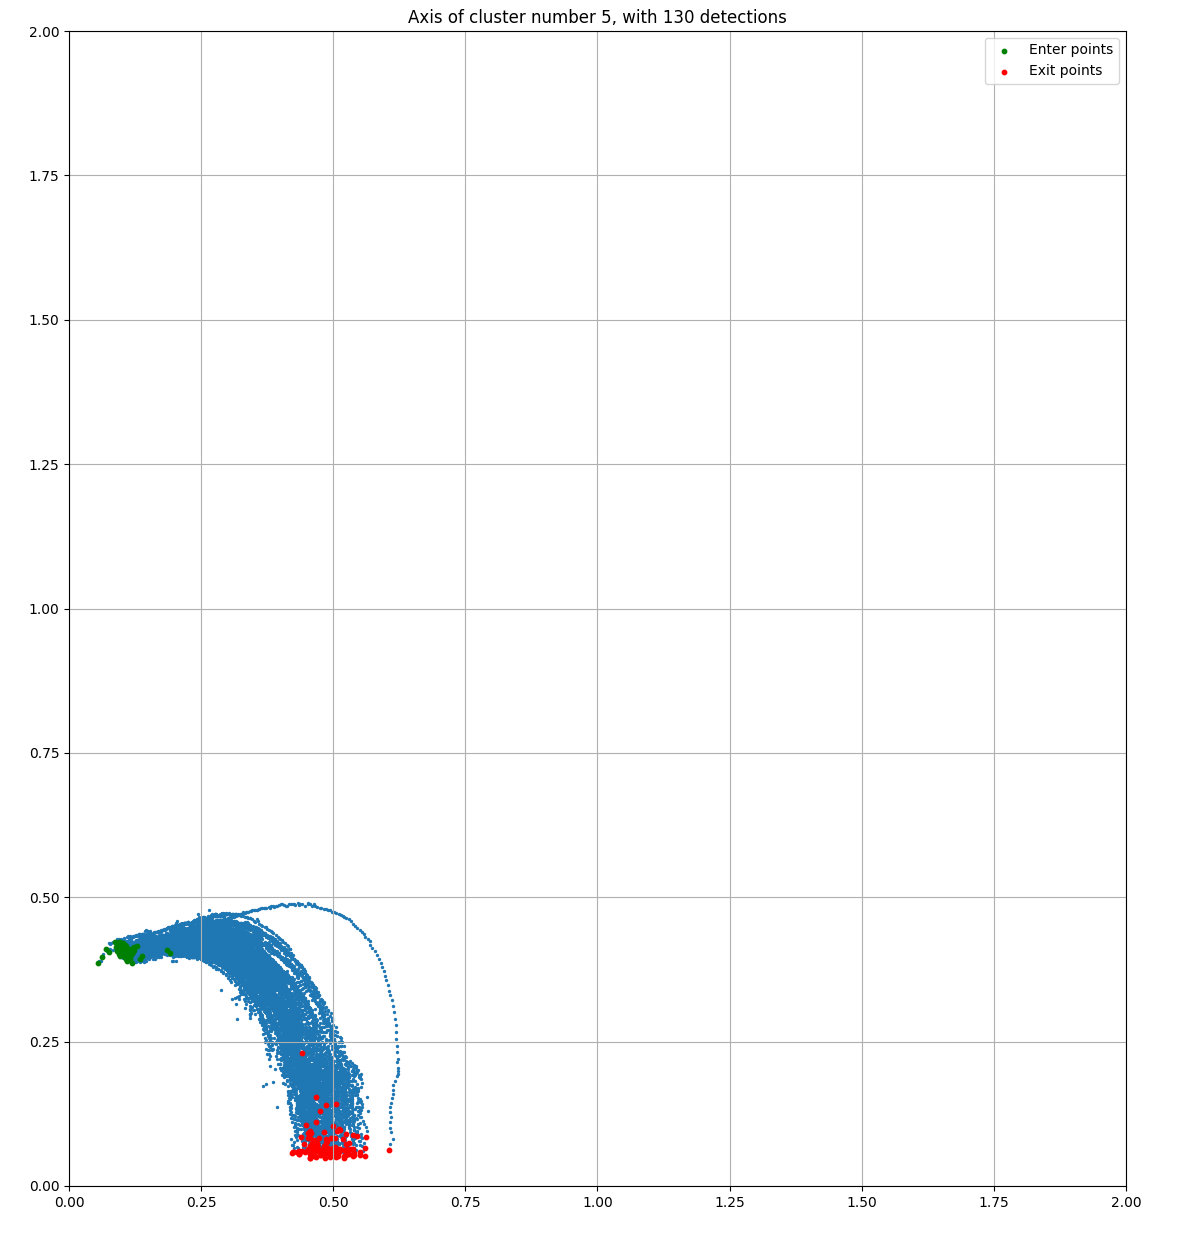
\includegraphics[scale=0.1]{../clustering/n_cluster_5_n_tracks_130_cropped.jpg}
        \end{figure}
    \end{columns}
\end{frame}


\subsection{Adatok tisztítása}
\begin{frame}{Adatok tisztítása}
    \begin{itemize}
        \item Több különböző zajforrás
        \begin{itemize}
            \item YOLO késői detektálás és követés (a járművet már csak akkor veszi észre amikor bennt van a kereszteződésben)
            \item YOLO fals detektálás (rendőrlámpát vagy táblát autónak néz)
            \item DeepSORT áttapadások (egymáshoz közel elhaladó járművek identitása felcserélődik)
        \end{itemize} 
        \item Megoldások
        \begin{itemize}
            \item Kép relatív széleinek megtalálása min-max kereséssel (az utakat nem biztos, hogy a kép szélétől széléig látjuk, hanem a kép közepétől kezdődve, ezt okozhatja egy nagy épület)
            \item Szűrés trajektóriák kezdő és végpontjainak euklideszi távolsága alapján
            \item Szűrés trajektóriák egymást követő detektálásai közötti távolságokkal
        \end{itemize} 
    \end{itemize}   
\end{frame}

\subsection{Zajos vs Szűrt}
\begin{frame}{Zajos vs Szűrt}
    \begin{figure}
        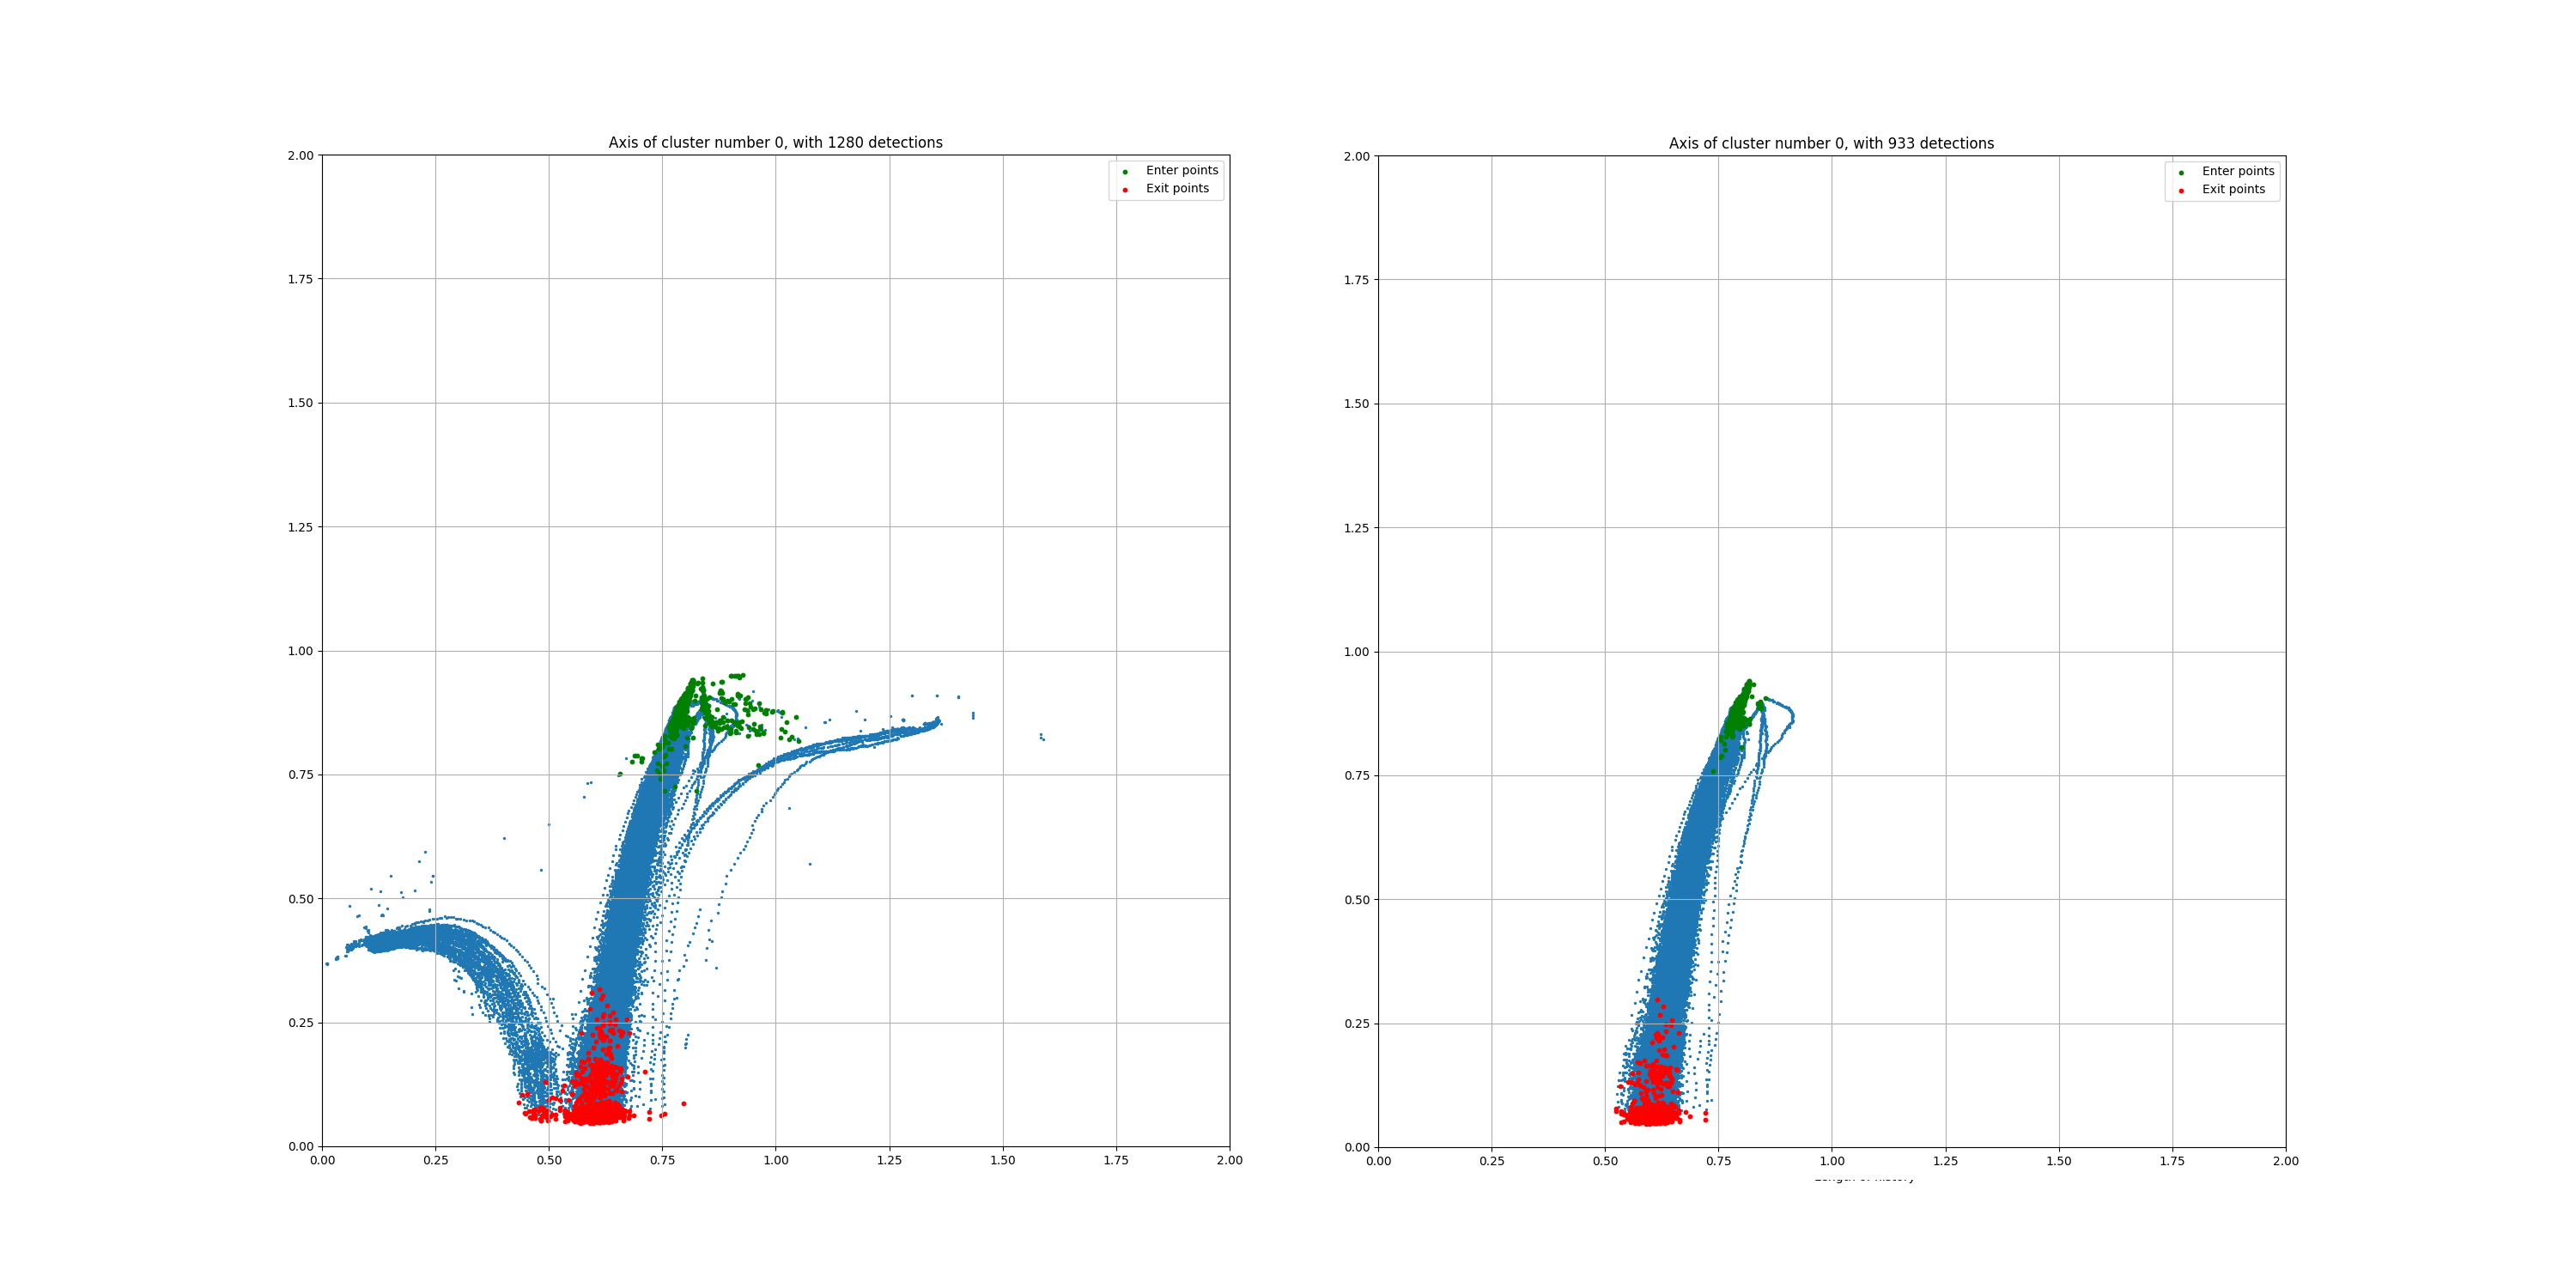
\includegraphics[scale=0.1]{../clustering/n_cluster_0_before_after.png}
        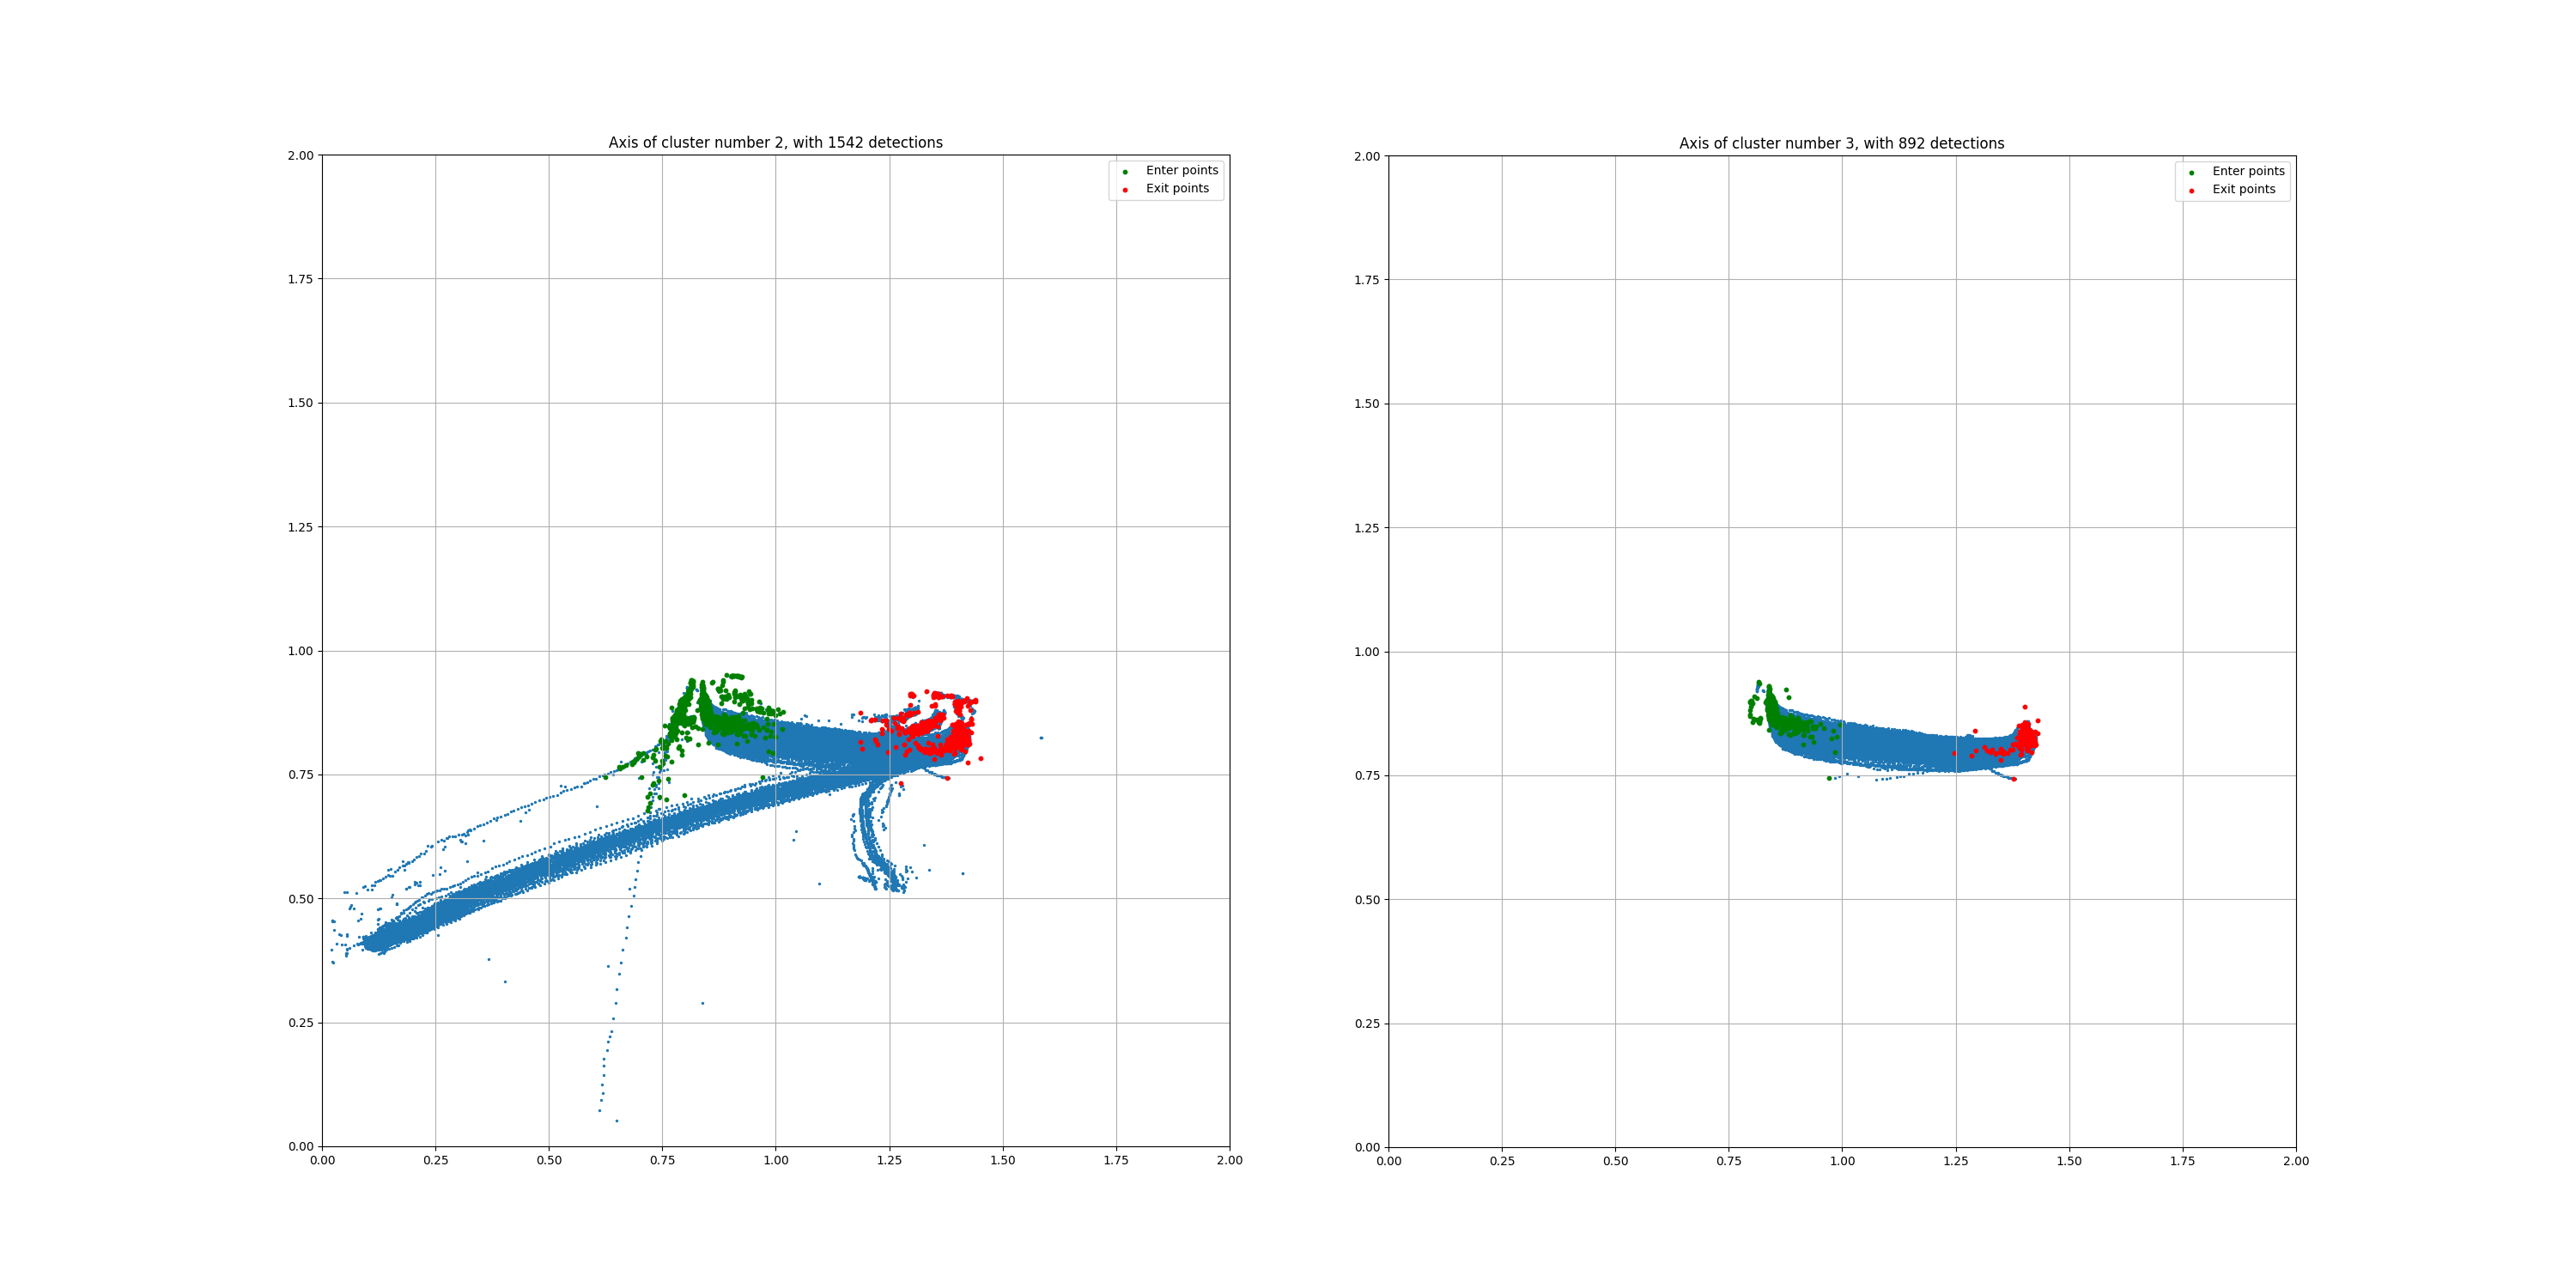
\includegraphics[scale=0.1]{../clustering/n_cluster_2_before_after.png}
    \end{figure}
\end{frame}

\subsection{OPTICS vs KMeans, BIRCH}
\begin{frame}{OPTICS vs KMeans, BIRCH}
    \begin{itemize}
        \item Klaszterezést nem triviális feladat
        \item Több algoritmus tesztelése
        \item KMeans, BIRCH, DBSCAN, OPTICS
        \item OPTICS adta a legjobb eredményeket
    \end{itemize}
    \begin{columns}
        \column{0.5\textwidth}
        \begin{figure}
            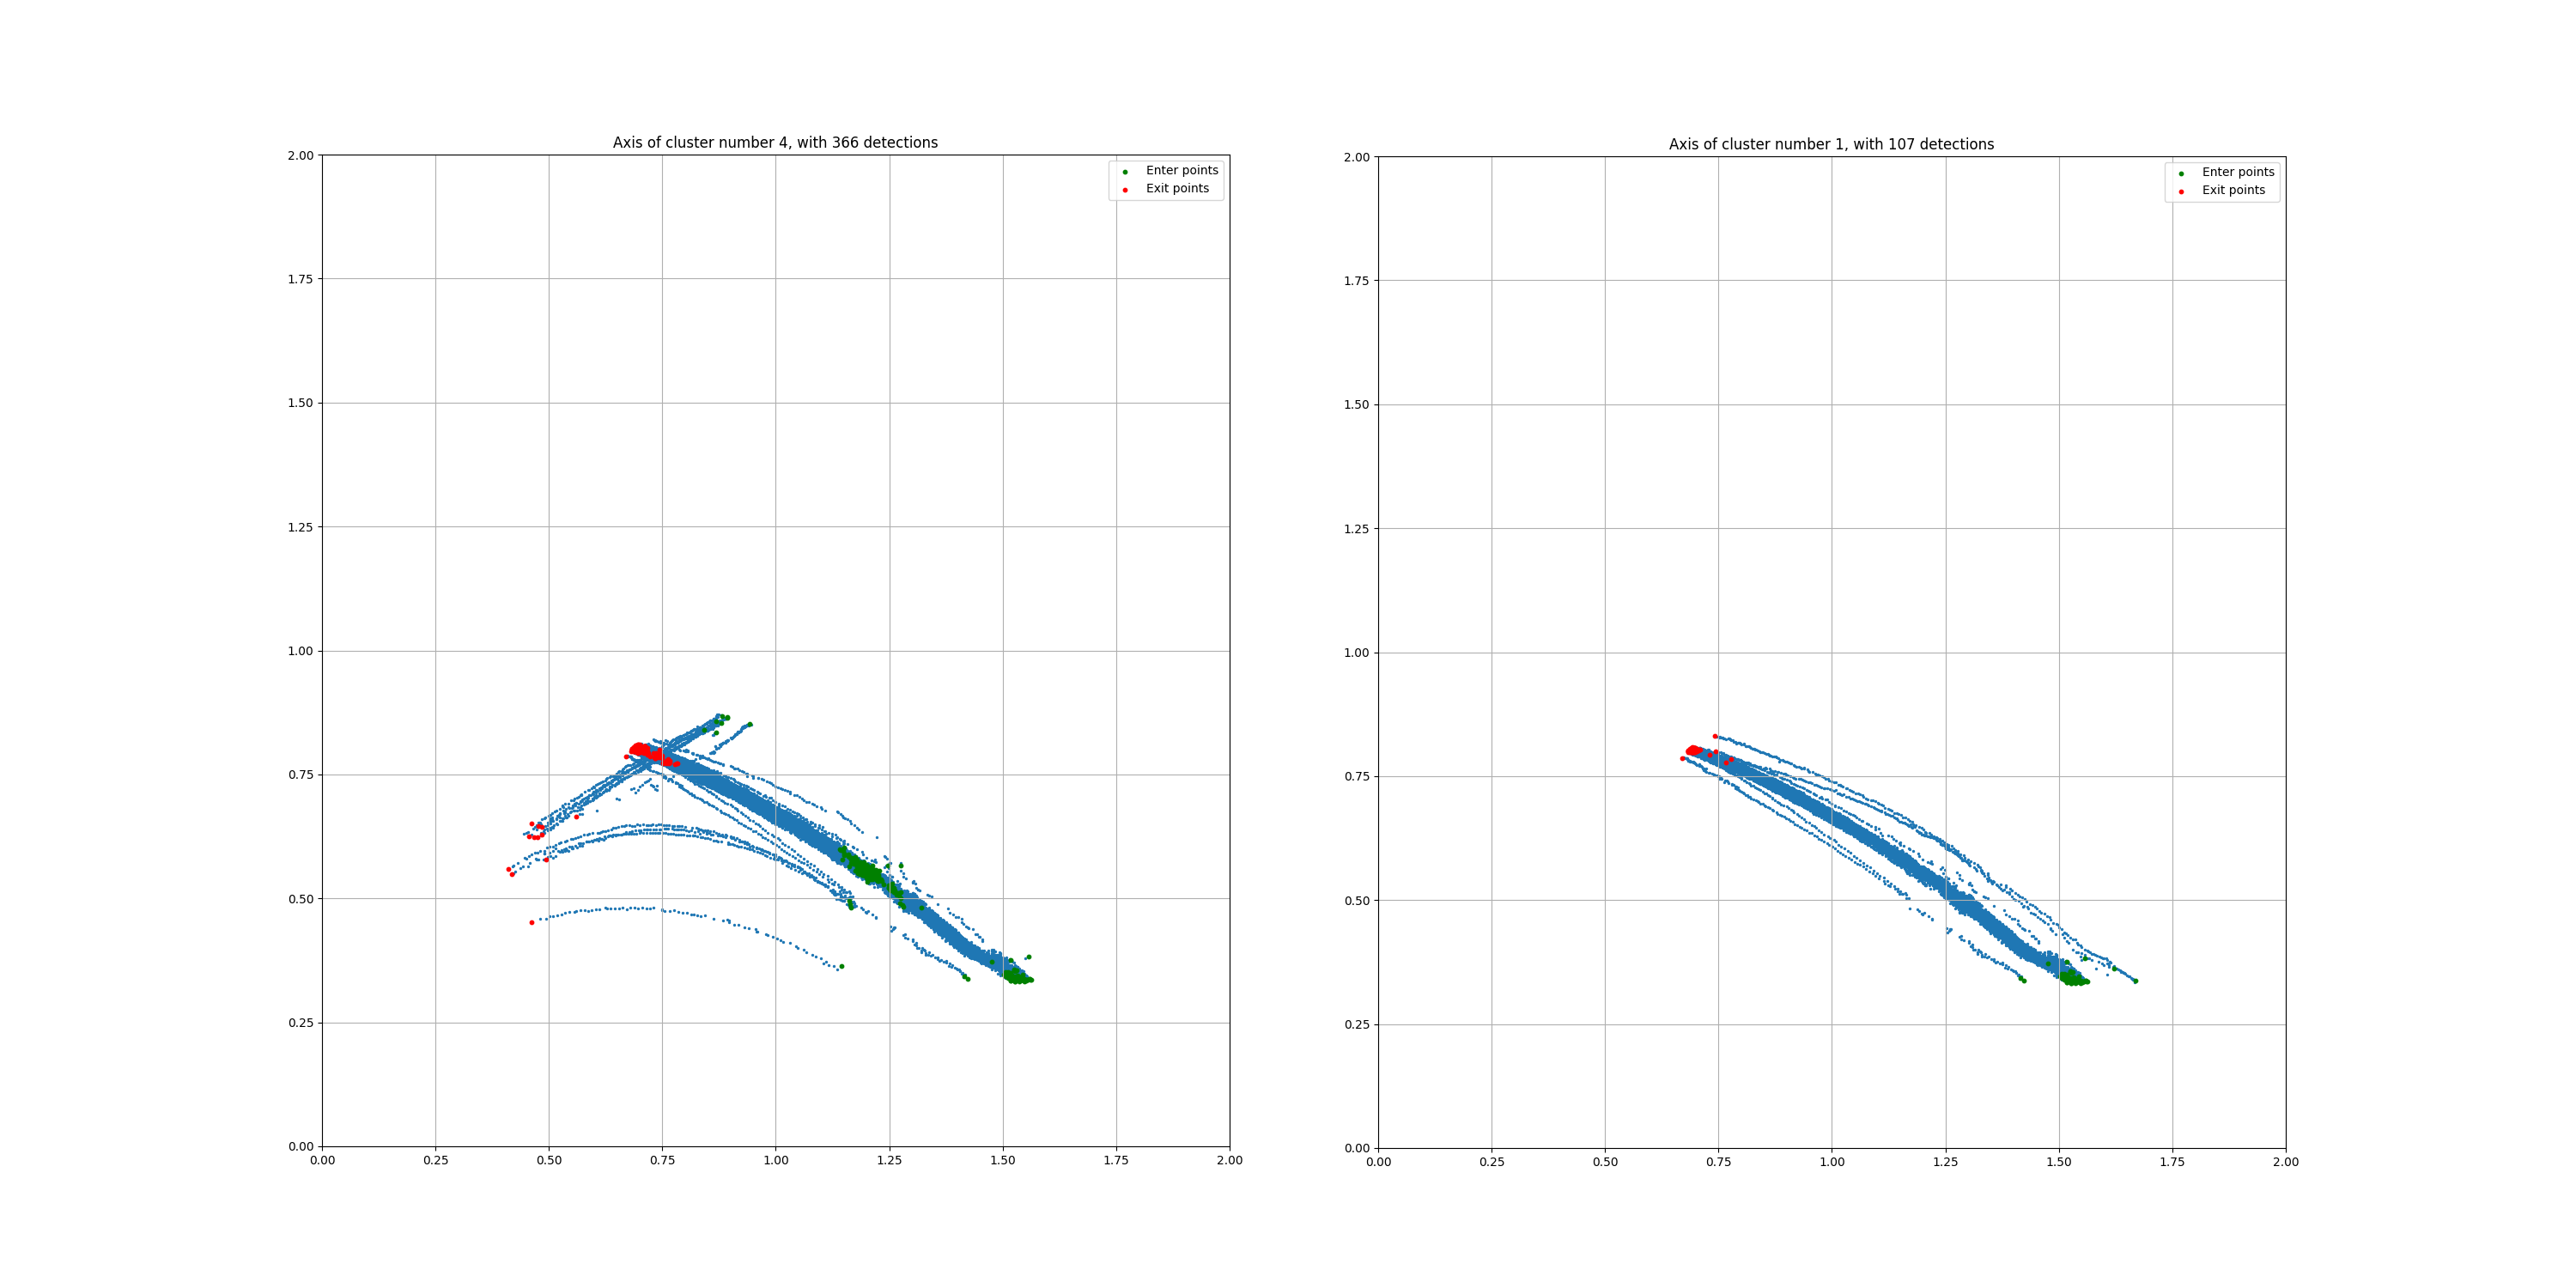
\includegraphics[scale=0.08]{../bad_clustering/example_kmeans_vs_optics.png}
        \end{figure}
        \column{0.5\textwidth}
        \begin{figure}
            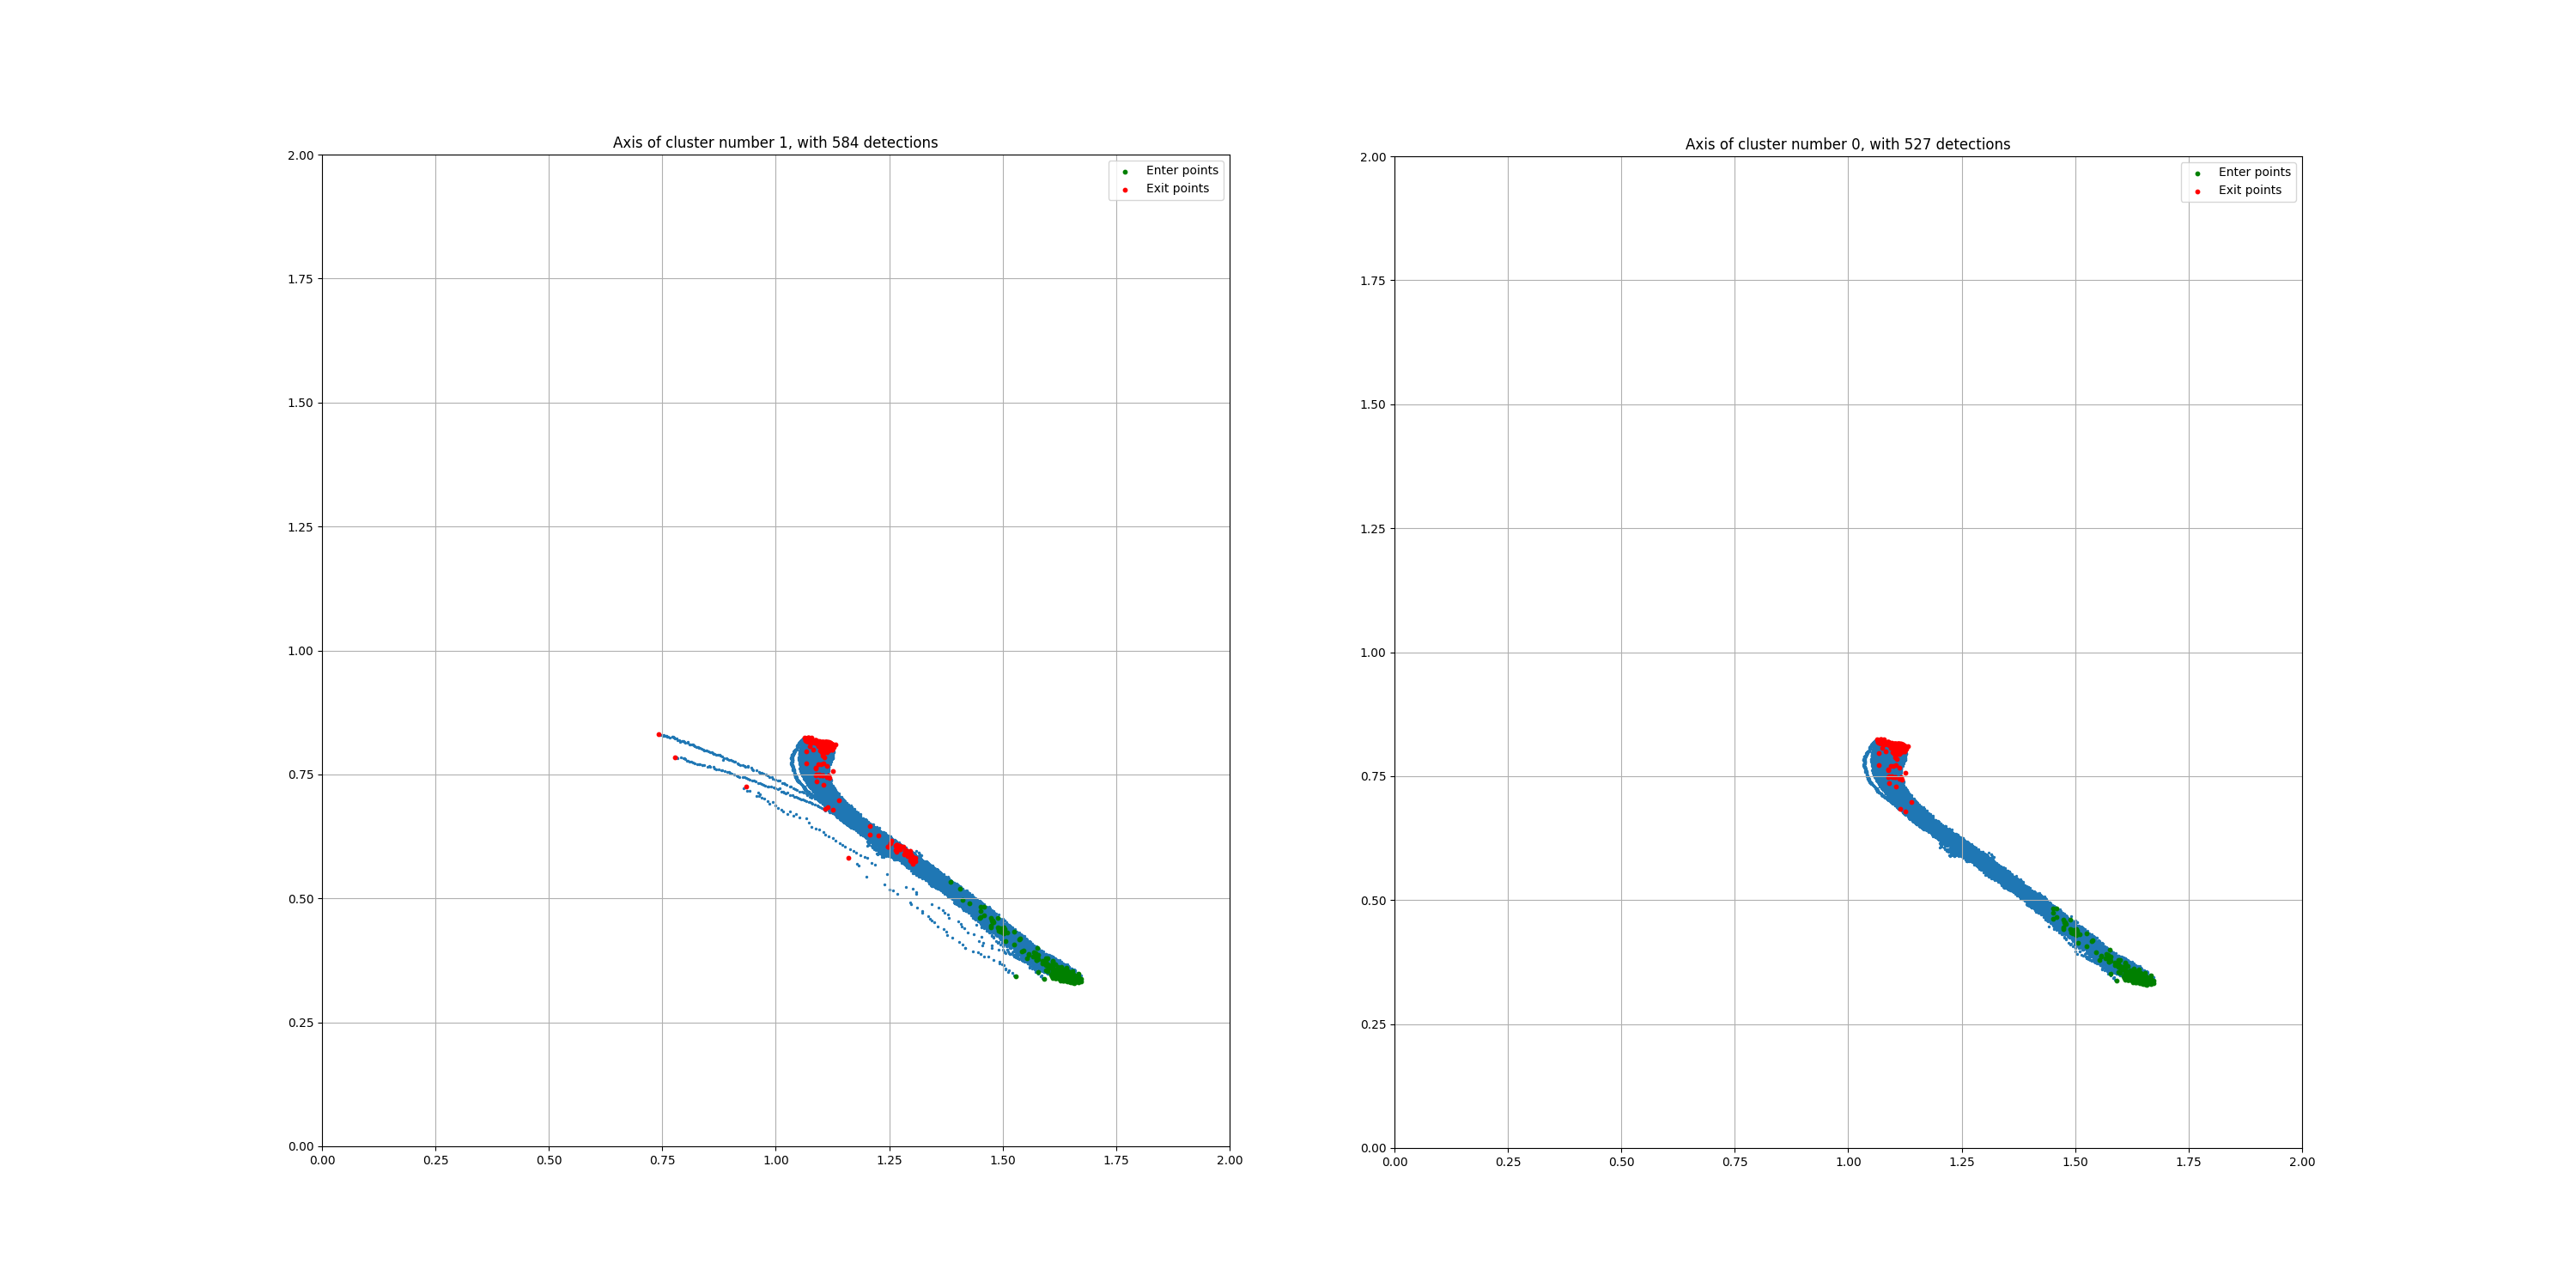
\includegraphics[scale=0.08]{../bad_clustering/example_birch_vs_optics.png}
        \end{figure}
    \end{columns}
\end{frame}

\subsection{OPTICS vs DBSCAN}
\begin{frame}{OPTICS vs DBSCAN}
    \centering
    \begin{figure}
        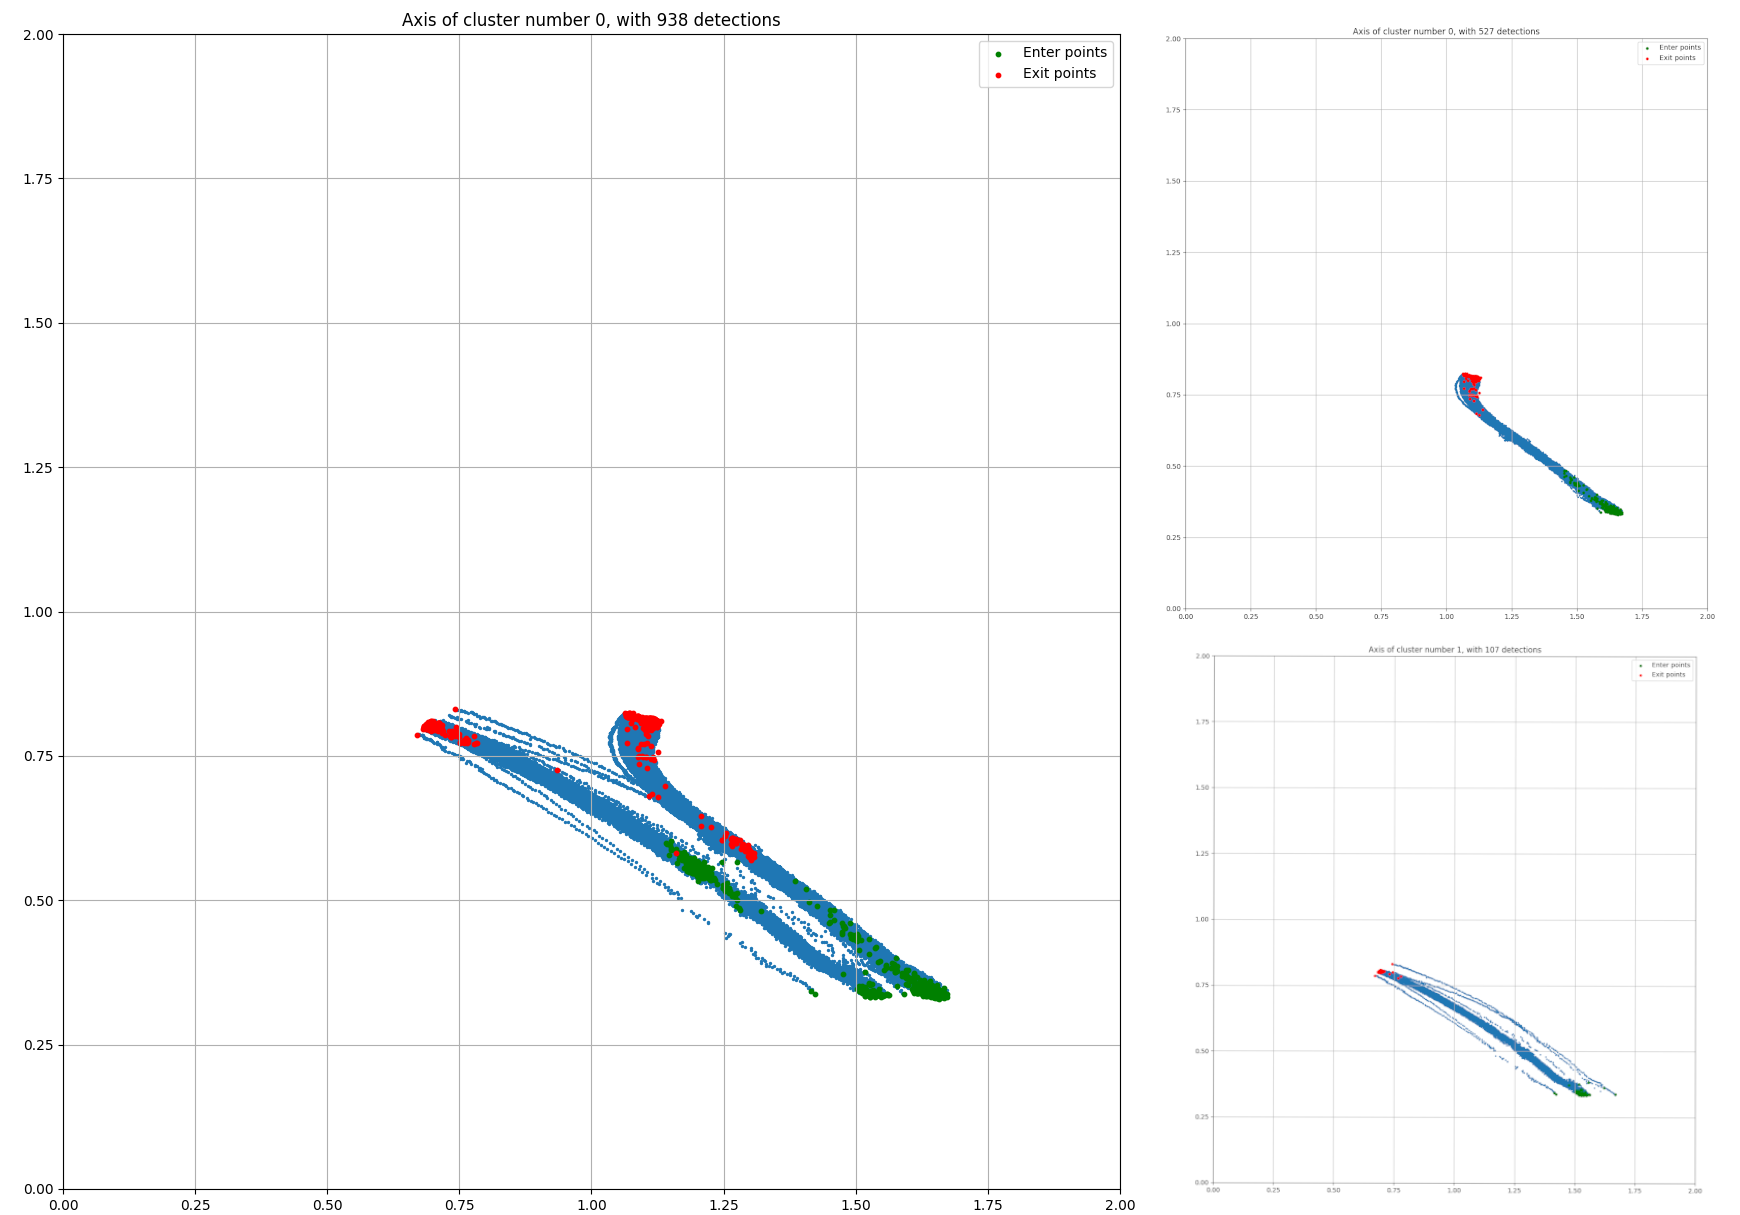
\includegraphics[scale=0.2]{../bad_clustering/example_dbscan_vs_optics_merged_cluster.png}
    \end{figure}
\end{frame}

\section{Klasszifikáció (Supervised)}
\begin{frame}{Klasszifikáció (Supervised)}
    \begin{itemize}
        \item Megfigyelt autó besorolása a klaszterezés alapján megfigyelt csoportba.
        \item Feature vektorok: trajektóriák felosztása több kisebb részre, amik valós idejű futásból származó trajektóriákhoz hasonlítanak
        \begin{itemize}
            \item v1: [kezdőkoordinátája, sebessége, középső koordinátája, utolsó koordinátája, sebessége]
            \item v7: [kezdőkoordinátája $\cdot 1$, sebessége $\cdot 100$, utolsó koordinátája $\cdot 2$, sebessége $\cdot 200$]
        \end{itemize}
        \item Adathalmaz dúsítása: egy trajektóriából több feature vektor generálása, tanító adathalmaz megnövelése
        \item Trajektóriák hossza: 15 és 30 hosszúságú trajektóriák tesztelése
        \item Eredmény: hossz növeléssel nem történik pontosságban javulás
    \end{itemize}
\end{frame}

\subsection{Klasszifikációs algoritmusok}
\begin{frame}{Klasszifikációs algoritmusok}
    \begin{itemize}   
        \item K-NearestNeighbors, SupportVectorMachine, DecisionTree 
        \item 5 különböző helyszín adatain mért pontosságok átlaga
        \item Top1: legvalószínűbb előrejelzés tényleg az elvárt osztály
        \item Top2: 2 legvalószínűbb előrejelzésben benne van az elvárt osztály
    \end{itemize}
    \begin{table}[]
    \begin{tabular}{|lccc|}
    \hline
    \multicolumn{4}{|c|}{\begin{tabular}[c]{@{}c@{}}Average Accuracy Feature Vector v1\end{tabular}}    \\ \hline
    \hline
    \multicolumn{1}{|l|}{} & \multicolumn{1}{c|}{Balanced} & \multicolumn{1}{c|}{Top 1}   & Top 2   \\ \hline
    \multicolumn{1}{|l|}{\textcolor[rgb]{1,0,0}{KNN}}     & \multicolumn{1}{c|}{\textcolor[rgb]{1,0,0}{94.16\%}}  & \multicolumn{1}{c|}{\textcolor[rgb]{1,0,0}{96.71\%}} & \textcolor[rgb]{1,0,0}{99.46\%} \\ \hline
    \multicolumn{1}{|l|}{SVM}     & \multicolumn{1}{c|}{81.65\%}  & \multicolumn{1}{c|}{90.82\%} & 98.05\% \\ \hline
    \multicolumn{1}{|l|}{DT}      & \multicolumn{1}{c|}{93.11\%}  & \multicolumn{1}{c|}{94.88\%} & 96.03\% \\ \hline
    \end{tabular}
    %\caption{Testset Feature Vektor V1}
    %\label{table:2}
    \end{table}

    \begin{table}[]
    \begin{tabular}{|lccc|}
    \hline
    \multicolumn{4}{|c|}{\begin{tabular}[c]{@{}c@{}}Average Accuracy Feature Vector v7\end{tabular}}    \\ \hline
    \hline
    \multicolumn{1}{|l|}{} & \multicolumn{1}{c|}{Balanced} & \multicolumn{1}{c|}{Top 1}   & Top 2   \\ \hline
    \multicolumn{1}{|l|}{\textcolor[rgb]{1,0,0}{KNN}}     & \multicolumn{1}{c|}{\textcolor[rgb]{1,0,0}{92.08\%}}  & \multicolumn{1}{c|}{\textcolor[rgb]{1,0,0}{95.61\%}} & 98.66\% \\ \hline
    \multicolumn{1}{|l|}{SVM}     & \multicolumn{1}{c|}{88.72\%}  & \multicolumn{1}{c|}{93.86\%} & \textcolor[rgb]{1,0,0}{98.92\%} \\ \hline
    \multicolumn{1}{|l|}{DT}      & \multicolumn{1}{c|}{89.46\%}  & \multicolumn{1}{c|}{93.30\%} & 94.55\% \\ \hline
    \end{tabular}
    %\caption{Testset Feature Vektor V7 Stride 15}
    %\label{table:3}
    \end{table}
\end{frame}

\section{Megjelenítő Alkalmazás}
\begin{frame}{Megjelenítő Alkalmazás}
    \begin{itemize}
        \item Saját fejlesztésű megjeleítő alkalmazás
        \item Zöld: legvalószínűbb előrejelzés
        \item Piros: második legvalószínűbb előrejelzés
    \end{itemize}
    \centering
    \movie[showcontrols=true]{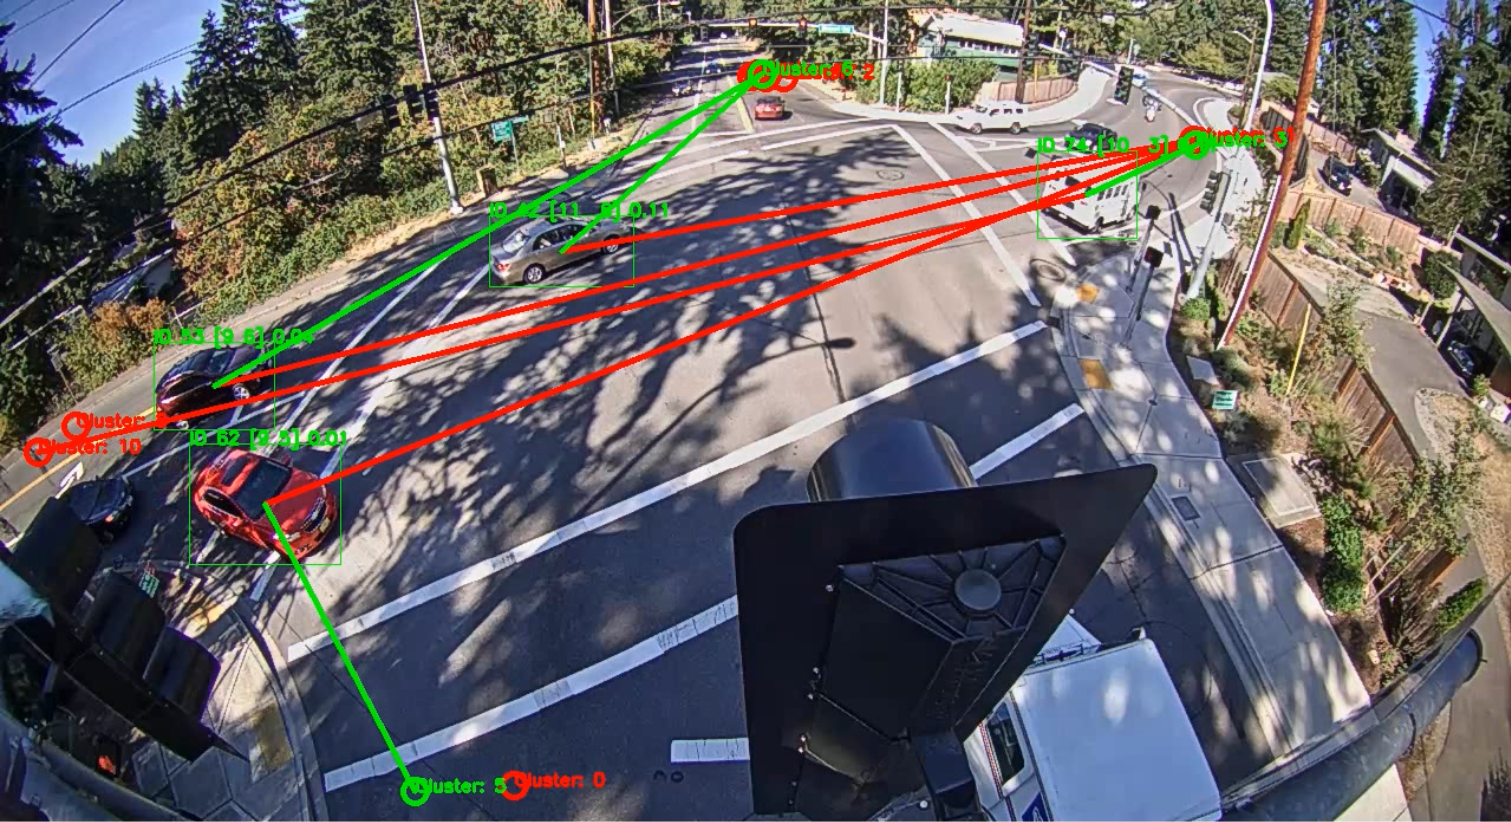
\includegraphics[scale=0.2]{../visualization/bellevue_newport.png}}{Newport_binary_KNN_n_neighbors_15_stride-15_v7.mp4}
\end{frame}

\section{Elmélet implementálása}
\begin{frame}{Elmélet implementálása}
    \begin{itemize}
        \item YOLOv7 és DeepSORT detektáló alkalmazásba integrálása
        \item SQL Adatbázis architektúra tervezése, implementálása
        \item Klaszterezés: Scikit-Learn
        \item Klasszifikáció: Scikit-Learn
        \item Klasszifikációs Modellek tárolása: Pickle, Joblib
        \item Megjelenítő alkalmazás
        \item Fejlesztői környezet: Linux, Python, Codium
        \item Saját forráskód mérete: 7460 sor
    \end{itemize}
\end{frame}


\end{document}